\documentclass[main.tex]{main.tex}

\pagestyle{empty}
\begin{document}

    \tikzset{edge from parent/.style=
            {draw, edge from parent path={(\tikzparentnode.south)
        -- +(0,-8pt)
        -| (\tikzchildnode)}},
        blank/.style={draw=none}}
    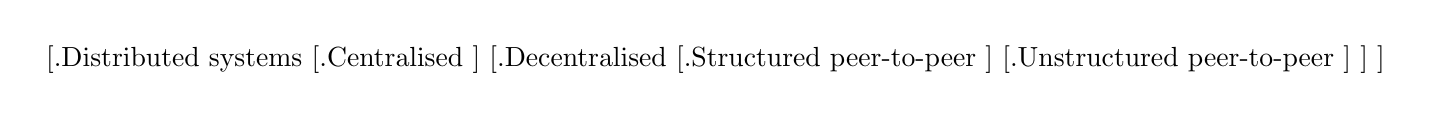
\begin{tikzpicture}
        \matrix
        {
            \node{\Tree
                [.{Distributed systems}
                    [.Centralised ]
                    [.Decentralised
                        [.{Structured peer-to-peer} ]
                        [.{Unstructured peer-to-peer} ]
                    ]
                ]
            };\\
        };
    \end{tikzpicture}

\end{document}
